\section{Proposed Approach}
\label{sec:approach}
% The input  (Figure \ref{fig_sysarch}) is a feature-based CAD model represented by  ($\cup_qf^3$), where `$\cup$' denotes a collection, of `$q$' features (`$f$') having dimensionality `$3$' (solids). In practice, the thin-walled CAD models come in various types, such as mesh, solid, feature-based CAD, etc. This research, as it leverages feature information \cite{YogeshCOEP2013}, expects a feature-based CAD model as input. This, at times can be deemed as limitation, in case of unavailability due to format restrictions, proprietary data etc. But, techniques such as segmentation, feature recognition (FR), can be used effectively to convert the non-feature-based model to a feature-based one.

The input (Figure \ref{fig_sysarch}) is a feature-based CAD model represented by $(\cup_q f^3)$, where $\cup$ denotes a collection of $q$ features ($f$) having dimensionality $3$ (solids). In practice, thin-walled CAD models can be available in various representations, such as mesh, solid, or feature-based CAD. This research, as it leverages feature information \cite{YogeshCOEP2013}, expects a feature-based CAD model as input. This may be considered a limitation in cases where such a representation is unavailable due to format restrictions or proprietary data. However, techniques like segmentation, feature recognition (FR), can be effectively used to convert a non-feature-based model to a feature-based one.

%\smallskip

% \begin{minipage}[c]{\linewidth}
    % \begin{minipage}[c]{0.45\linewidth}
\begin{itemize}[noitemsep,topsep=2pt,parsep=2pt,partopsep=2pt,leftmargin=*]
%\item \textbf{Input}: Feature-based CAD models, which are widely available in most of the commercial CAD applications. It is represented by  ($\cup_qf^3$), where `$\cup$' denotes a collection, of `$q$' features (`$f$') having dimensionality `$3$' (solids). Thin-walled CAD models come in various representations, such as mesh, solid, feature-based, etc. This research expects a feature-based CAD model, which can be deemed as limitation in case of its unavailability. But, techniques, such as segmentation, decomposition, feature recognition (FR), etc. can convert a non-feature-based representation to the feature-based CAD model.

	\begin{figure}[ht]
	\centering 
	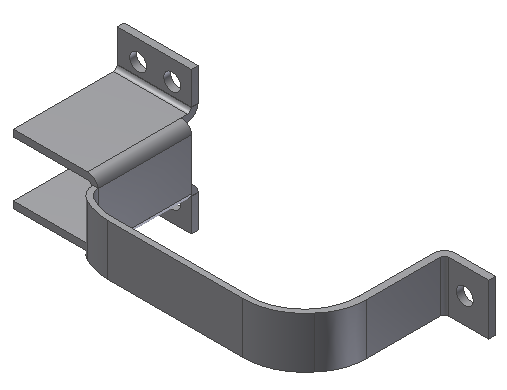
\includegraphics[width=0.5\linewidth]{images/nonCellularBracket}
	\captionof{figure}{Original Part}
	\label{fig_orig}
	\end{figure}
	
\item \textbf{Defeaturing ($\cup_rf^3, r \leq q$) }:  % Computes gross shape by removing irrelevant/superficial features \cite{YogeshIITM2013}, using Feature taxonomy and size-based Remnant feature approach (\cite{YogeshCADConf2015}). 
Computes the gross shape by removing irrelevant or superficial features \cite{YogeshIITM2013}, using Feature taxonomy and a size-based Remnant feature approach (\cite{YogeshCADConf2015}).

\item \textbf{Generalization ($\cup_rL^3$) }: %``ABEL'' transforms form-features to ``Loft/Sweep'' representations ($L$), making it simpler to develop a generic, portable algorithm (\cite{YogeshIITG2014}). 
The 'ABEL' transform converts form-features to Loft/Sweep' representations ($L$), simplifying the development of a generic, portable algorithm (\cite{YogeshIITG2014}).

\item \textbf{Decomposition}: Cellular decomposition is performed at each feature step to form a graph of nodes containing non-volumetrically overlapping cellular bodies with their respective owner-Sweep feature.

	\begin{figure}[ht]
	\centering 
	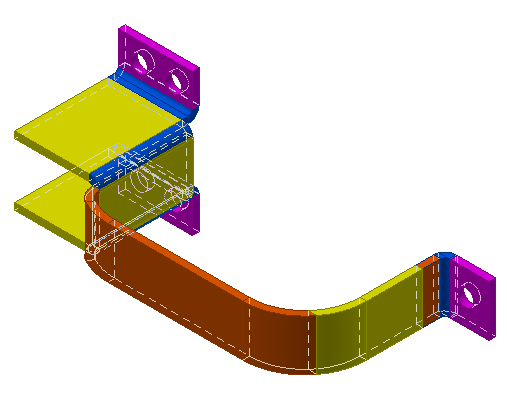
\includegraphics[width=0.5\linewidth]{images/CellularBracket}
	\captionof{figure}{Decomposition}
	\label{fig_cd}
	\end{figure}
	
	\begin{figure}[ht]
	\centering 
	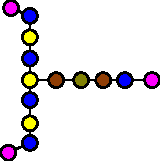
\includegraphics[width=0.4\linewidth]{images/CellGraphBracket.pdf}
	\captionof{figure}{Graph}
	\label{fig_cg}
	\end{figure}	
	
\item \textbf{Midsurface Computation}: Using the topology of the graph, nodes are classified into midsurface-patch generating nodes (solid cells - $sCell$s) and interaction-resolving nodes (interface cells - $iCell$s). The midsurface patch is computed by first extracting the profile and guide curve from the owner Sweep feature, then either offsetting the profile for shorter guide curves or sweeping the midcurve \cite{YogeshETES2014,YogeshIJCAET2017} along the guide curve.

	\begin{figure}[ht]
	\centering 
	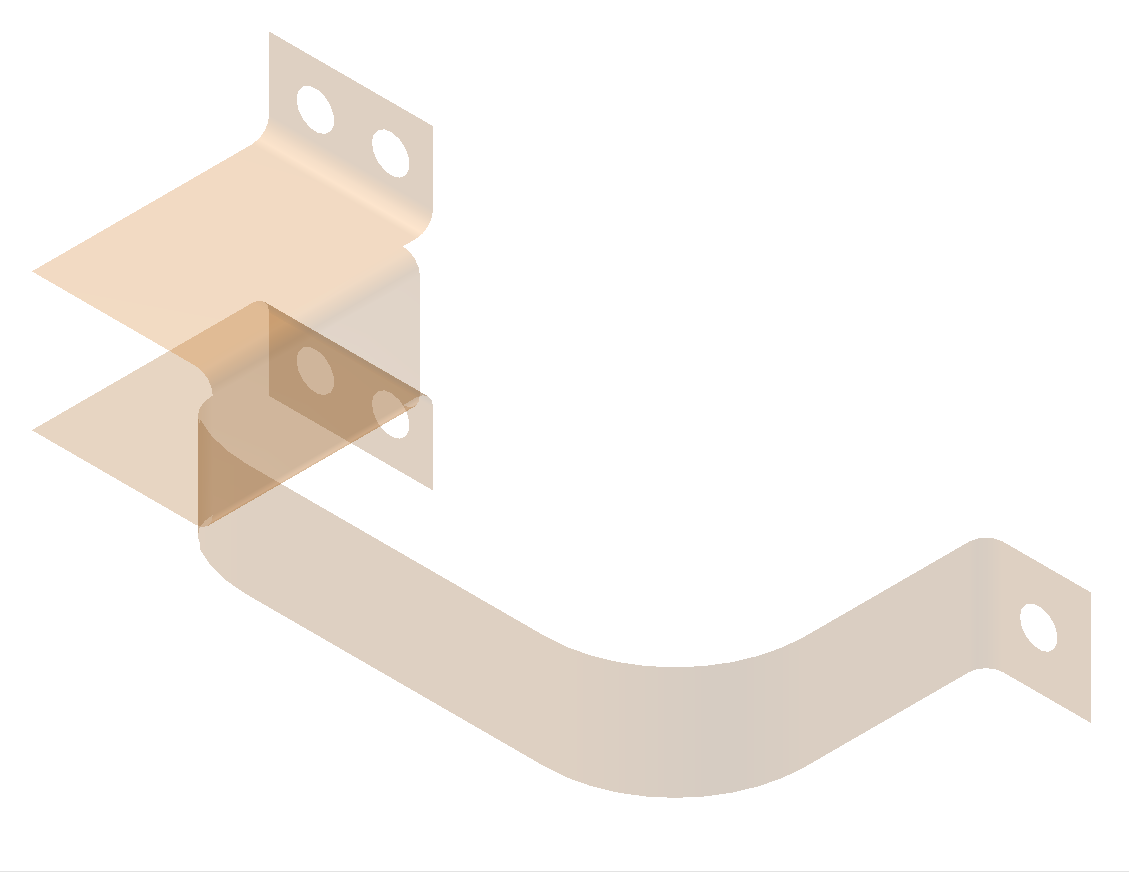
\includegraphics[width=0.5\linewidth]{images/MidsurfAfterDormant}
	\captionof{figure}{Midsurface}
	\label{fig_mids}
	\end{figure}	
	
\item \textbf{Validation}: The midsurface must faithfully mimic the input shape. A novel topological method is used to validate the correctness of the midsurface (\cite{YogeshCADandA2015}).

%\item \textbf{Output}: A well-connected output midsurface is then sent to downstream applications such as CAE analysis.
\end{itemize}

% \begin{figure}[htp]
% \centering     %%% not \center
% \subfloat[Original Part]{\label{fig_orig}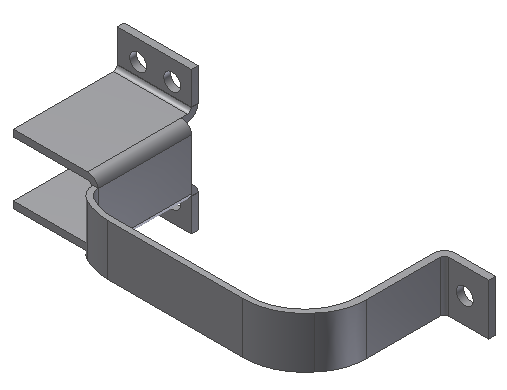
\includegraphics[width=0.23\linewidth,valign=t]{images/nonCellularBracket}} \quad
% \subfloat[Decomposition]{\label{fig_cd}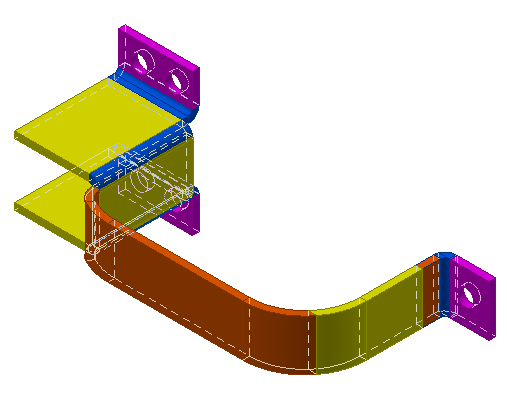
\includegraphics[width=0.23\linewidth,valign=t]{images/CellularBracket}}\quad
% \subfloat[Graph]{\label{fig_cg}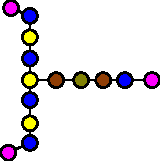
\includegraphics[width=0.175\linewidth,valign=t]{images/CellGraphBracket.pdf}} \quad
% \subfloat[Midsurface]{\label{fig_mids}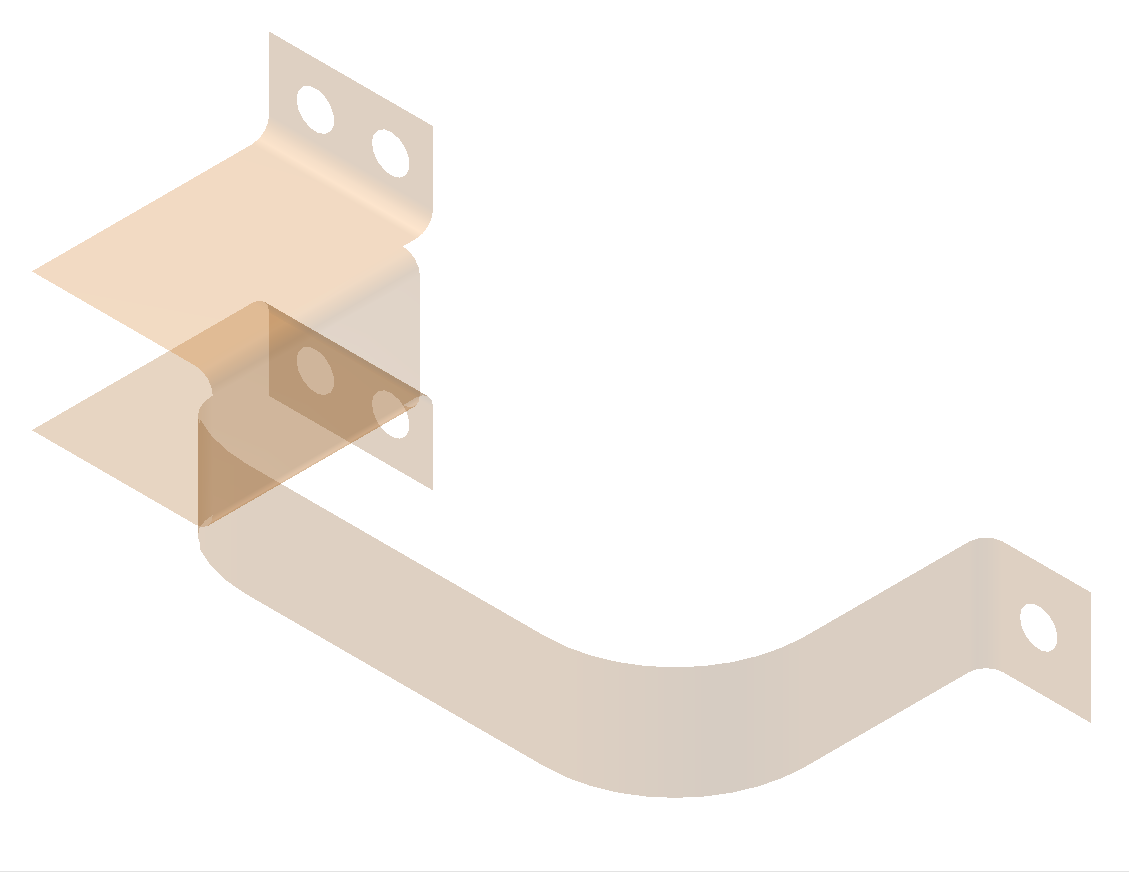
\includegraphics[width=0.23\linewidth,valign=t]{images/MidsurfAfterDormant}}
% \end{figure}

    % \end{minipage}
    % \hfill
    % \begin{minipage}[c]{0.5\linewidth}
	\begin{figure}[ht]
	\centering 
	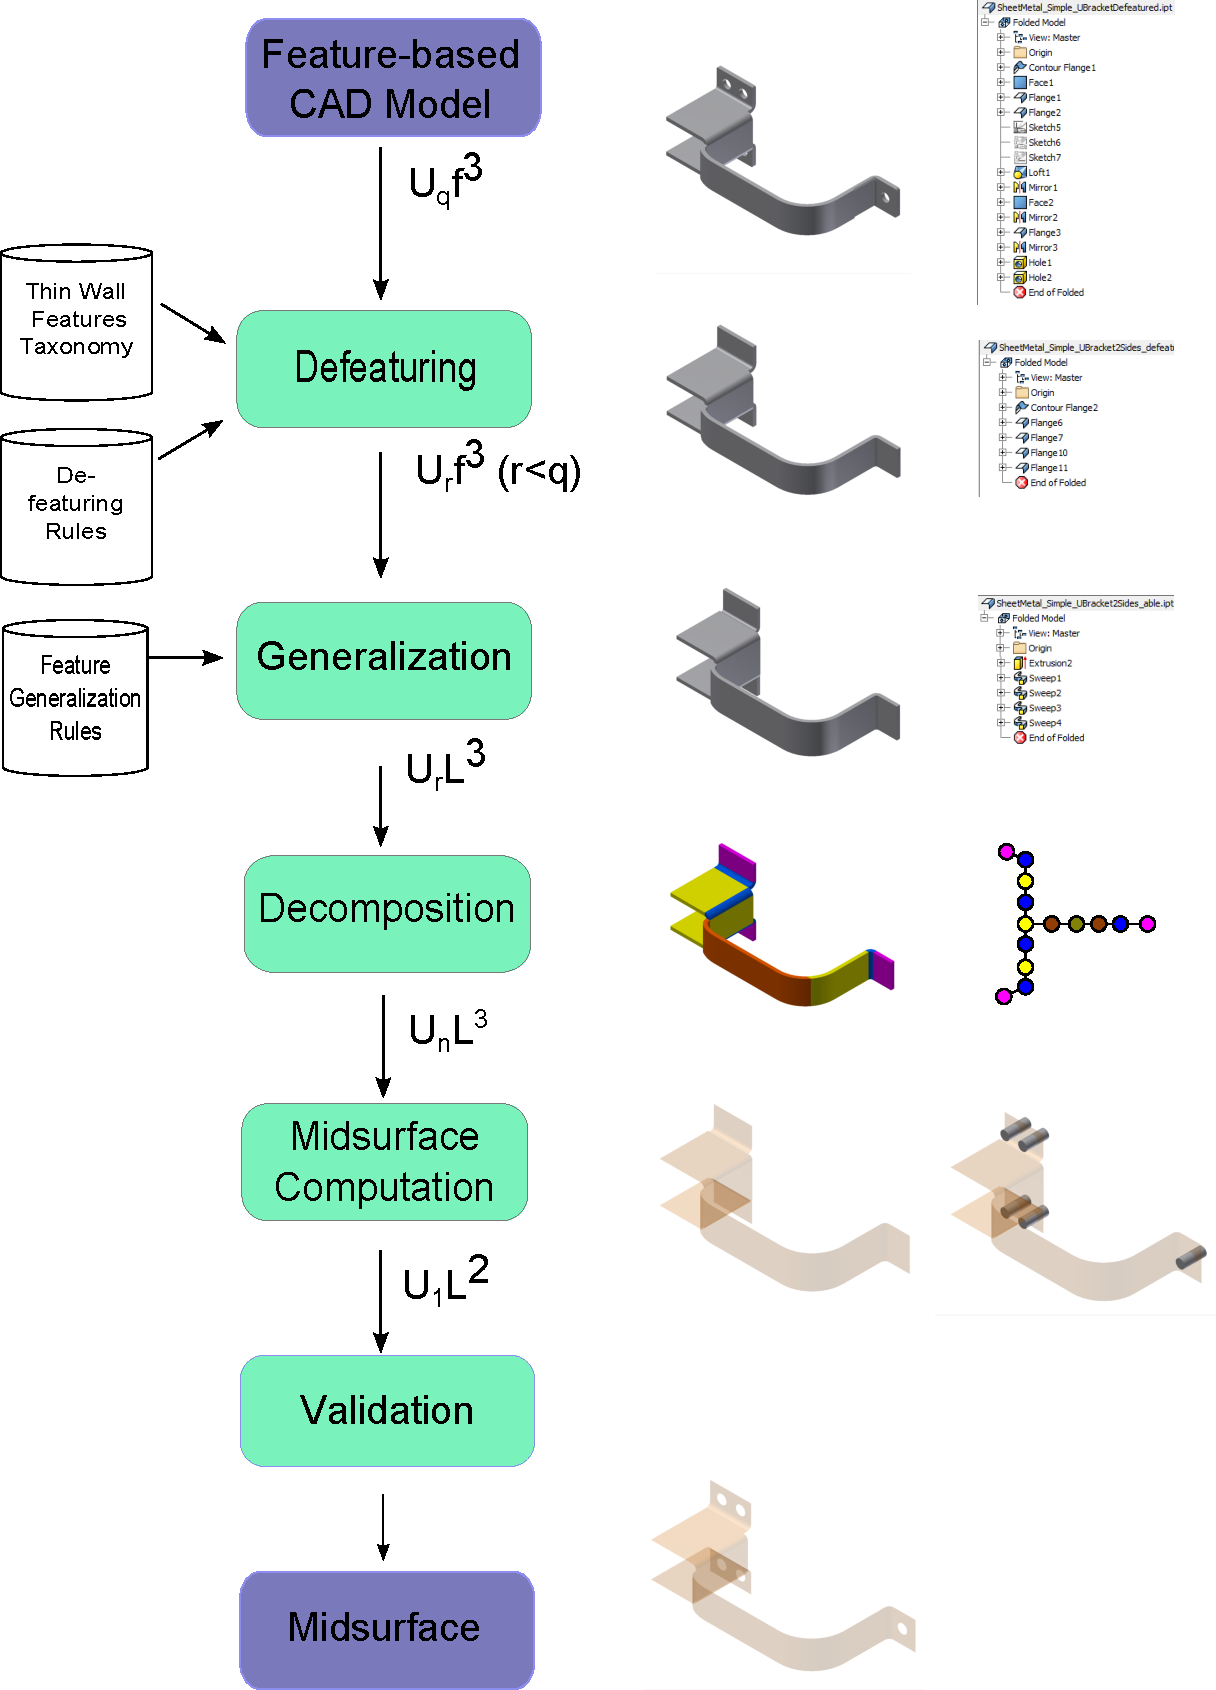
\includegraphics[width=0.95\linewidth]{images/SystemArchitecture3.pdf}
	\captionof{figure}{Overall work-flow}
	\label{fig_sysarch}
	\end{figure}
    % \end{minipage}

% \end{minipage}    

% A well-connected output midsurface is then sent to downstream applications such as CAE analysis. 

%\bigskip


The following is a comparative analysis of some relevant approaches vis-à-vis the proposed approach:

\begin{enumerate}
    \item Chong et al. \cite{Chong2004}: Uses concave edge decomposition. Midcurves by collapsing edge pairs. If they form a loop, creates a midsurface patch. Problems: Hard-coded inequalities/values to detect edge-pairs. Connection logic is not generic and comprehensive. In comparison, the proposed approach: A generic treatment for the computation of midcurves, midsurface patches and their connections
    \item Boussuge et al. \cite{Boussuge2014}: Generative decomposition. Recognizes Extrudes of each sub-volume. Creates midsurface patches in each and connects them together. Problems: No fillets/chamfers, only Additive cells, only Extrudes with Analytical surfaces, expensive MAT to detect thin profiles and works only on Parallel and Orthogonal connections, but the proposed approach: No such restriction, Re-inserts -ve cells, Generic Sweep extend-able to Loft, Simple rules of size of profile/guide, Generic logic for any numbers/types of connections.
\end{enumerate}